% Created 2024-06-30 Sun 15:11
% Intended LaTeX compiler: xelatex
\documentclass[11pt]{article}
\usepackage{hyperref}
% TIPS
% \substack{a\\b} for multiple lines text





% pdfplots will load xolor automatically without option
\usepackage[dvipsnames]{xcolor}

\usepackage{forest}
% two-line text in node by [two \\ lines]
% \begin{forest} qtree, [..] \end{forest}
\forestset{
  qtree/.style={
    baseline,
    for tree={
      parent anchor=south,
      child anchor=north,
      align=center,
      inner sep=1pt,
    }}}
%\usepackage{flexisym}
% load order of mathtools and mathabx, otherwise conflict overbrace

\usepackage{mathtools}
%\usepackage{fourier}
\usepackage{pgfplots}
\usepackage{amsthm, mathabx,  amsmath, commath}
\usepackage{amsfonts}

\usepackage{empheq}
\usepackage{tikz}
\usetikzlibrary{arrows.meta}
\usepackage[most]{tcolorbox}

\newtheorem{theorem}{Theorem}[section]
\newtheorem{definition}{Definition}[section]
\newtheorem{corollary}{Corollary}[section]
\newtheorem{example}{Example}[section]
\newtheorem{lemma}{Lemma}[section]
\newtheorem{proposition}{Proposition}[section]

\newcommand{\bl}[1] {\boldsymbol{#1}}
\newcommand{\Wt}[1] {\stackrel{\sim}{\smash{#1}\rule{0pt}{1.1ex}}}
\newcommand{\wt}[1] {\widetilde{#1}}


%For boxed texts in align, use Aboxed{}
%otherwise use boxed{}

\DeclareMathSymbol{\widehatsym}{\mathord}{largesymbols}{"62}
\newcommand\lowerwidehatsym{%
  \text{\smash{\raisebox{-1.3ex}{%
    $\widehatsym$}}}}
\newcommand\fixwidehat[1]{%
  \mathchoice
    {\accentset{\displaystyle\lowerwidehatsym}{#1}}
    {\accentset{\textstyle\lowerwidehatsym}{#1}}
    {\accentset{\scriptstyle\lowerwidehatsym}{#1}}
    {\accentset{\scriptscriptstyle\lowerwidehatsym}{#1}}
}

\usepackage{graphicx}
    
% text on arrow for xRightarrow
\makeatletter
%\newcommand{\xRightarrow}[2][]{\ext@arrow 0359\Rightarrowfill@{#1}{#2}}
\makeatother


\def \bx {\boldsymbol{x}}
\def \ba {\boldsymbol{a}}
\def \bI {\boldsymbol{I}}
\def \bt {\boldsymbol{t}}
\def \bb {\boldsymbol{b}}
\def \bA {\boldsymbol{A}}
\def \bX {\boldsymbol{X}}
\def \bu {\boldsymbol{u}}
\def \bS {\boldsymbol{S}}
\def \bZ {\boldsymbol{Z}}
\def \bz {\boldsymbol{z}}
\def \by {\boldsymbol{y}}
\def \bw {\boldsymbol{w}}
\def \bT {\boldsymbol{T}}
\def \bS {\boldsymbol{S}}
\def \bm {\boldsymbol{m}}
\def \bW {\boldsymbol{W}}
\def \bY {\boldsymbol{Y}}
\def \bH {\boldsymbol{H}}
\def \blambda {\boldsymbol{\lambda}}
\def \bPhi {\boldsymbol{\Phi}}
\def \btheta {\boldsymbol{\theta}}
\def \bmu {\boldsymbol{\mu}}
\def \bphi {\boldsymbol{\phi}}
\def \bSigma {\boldsymbol{\Sigma}}
\def \lb {\left\{}
\def \rb {\right\}}
\def \caln {\mathcal{N}}
\def \dissum {\displaystyle\Sigma}
\def \dispro {\displaystyle\prod}
\def \E {\mathbb{E}}
\def \Q {\mathbb{Q}}
\def \V {\mathbb{V}}
\def \R {\mathbb{R}}
\def \calq {\mathcal{Q}}
\def \calg {\mathcal{G}}
\def \caln {\mathcal{N}}
\def \calr {\mathcal{R}}
\def \calm {\mathcal{M}}
\def \calc {\mathcal{C}}
\def \bcup {\bigcup}

\graphicspath{{../../books/}}
\makeindex

%% ox-latex features:
%   !announce-start, !guess-pollyglossia, !guess-babel, !guess-inputenc, caption,
%   image, !announce-end.

\usepackage{capt-of}

\usepackage{graphicx}

%% end ox-latex features


\author{Nancy Lynch}
\date{\today}
\title{Distributed Algorithms}
\hypersetup{
 pdfauthor={Nancy Lynch},
 pdftitle={Distributed Algorithms},
 pdfkeywords={},
 pdfsubject={},
 pdfcreator={Emacs 31.0.50 (Org mode 9.8-pre)}, 
 pdflang={English}}
\begin{document}

\maketitle
\tableofcontents

\section{Modelling \rom{2}: Asynchronous System Model}
\label{sec:orge26adf7}
\subsection{I/O Automata}
\label{sec:org3862f31}
A \textbf{signature} \(S\) is a triple consisting of three disjoint sets of actions: the \textbf{input actions},
\(in(S)\), the \textbf{output actions}, \(out(S)\), and the \textbf{internal actions}, \(int(S)\). We define the
\textbf{external actions}, \(ext(S)\), to be \(in(S)\cup out(S)\); and \textbf{locally controlled actions}, \(local(S)\)
to be \(out(S)\cup int(S)\); and \(acts(S)\) to be all the actions of \(S\). The \textbf{external signature},
\(extsig(S)\), is defined to be the signature \((in(S),out(S),\emptyset)\).

An \textbf{I/O automaton} \(A\), which we also call simply an \textbf{automaton}, consists of five components:
\begin{itemize}
\item \(sig(A)\), a signature
\item \(states(A)\)
\item \(start(A)\), a nonempty subset of \(states(A)\) known as the \textbf{start states} or \textbf{initial states}
\item \(trans(A)\), a \textbf{state-transition relation} where \(trans(A)\subseteq states(A)\times
          acts(sig(A))\times states(A)\).
\item \(tasks(A)\), a \textbf{task partition}, which is an equivalence relation on \(local(sig(A))\) having at most
countably many equivalence classes
\end{itemize}

We use \(acts(A)\) as shorthand for \(acts(sig(A))\), and similarly \(in(A)\), and so on.

We call an element \((s,\pi,s')\) of \(trans(A)\) a \textbf{transition}, or \textbf{step}, of \(A\). The transition
\((s,\pi,s')\) is called  an \textbf{input transition}, \textbf{output transition}, and so on, based on whether the
action \(\pi\) is an input action, output action, and so on.

If for a particular state \(s\) and action \(\pi\), \(A\) has some transition of the form
\((s,\pi,s')\), then we say that \(\pi\) is \textbf{enabled} in \(s\). Since every input action is required to
be enabled in every state, automata are said to be \textbf{input-enabled}. We say that state \(s\) is \textbf{quiescent}
if the only actions that are enabled in s are input actions.

A task \(C\) is \textbf{enabled} in a state \(s\) means somes action in \(C\) is enabled in \(s\).

\begin{examplle}[Channel I/O automaton]
\label{8.1.1}
Consider a communication channel automaton \(C_{i,j}\). Let \(M\) be a fixed message alphabet.
\begin{itemize}
\item \textbf{Signature}:
\begin{alignat*}{2}
&\text{Input}:\hspace{3cm}&&\text{Output:}\\
&\quad send(m)_{i,j},m\in M&&\quad receive(m)_{i,j},m\in M
\end{alignat*}
\item \textbf{States}: \(queue\), a FIFO queue of elements of \(M\), initially empty
\item \textbf{Transitions}:
\begin{alignat*}{2}
&send(m)_{i,j}\hspace{3cm}&&receive(m)_{i,j}\\
&\quad\text{Effect:}&&\quad\text{Precondition:}\\
&\quad\quad\text{add }m\text{ to }queue&&\quad\quad m\text{ is first on }queue\\
&&&\quad\text{Effect:}\\
&&&\quad\quad\text{remove first element of }queue
\end{alignat*}
\item \textbf{Tasks}: \(\{receive(m)_{i,j}:m\in M\}\)
\end{itemize}
\end{examplle}

\begin{examplle}[Process I/O automata]
\label{8.1.2}

Consider a process automaton \(P_i\). \(V\) is a fixed value set, \(null\) is a special value not in \(V\), \(f\) is a fixed function,
\(f:V^n\to V\)
\begin{itemize}
\item \textbf{Signature}:
\begin{itemize}
\item Input:
\begin{itemize}
\item \(init(v)_i,v\in V\)
\item \(receive(v)_{j,i}\), \(v\in V\), \(1\le j\le n\), \(j\neq i\)
\end{itemize}
\item Output:
\begin{itemize}
\item \(decide(v)_i\), \(v\in V\)
\item \(send(v)_{i,j}\), \(v\in V\), \(1\le j\le n\), \(j\neq i\)
\end{itemize}
\end{itemize}
\item \textbf{States}: \(val\), a vector indexed by \(\{1,\dots,n\}\) of elements in \(V\cup\{null\}\), all
initially \(null\)
\item \textbf{Transitions}:
\begin{alignat*}{2}
&init(v)_i,v\in V\hspace{2cm}&&receive(v)_{j,i},v\in V\\
&\quad\text{Effect:}&&\quad\text{Effect:}\\
&\quad\quad val(i):=v&&\quad\quad val(j):=v\\\\
&send(v)_{i,j}, v\in V&&decide(v)_i,v\in V\\
&\quad\text{Precondition:}&&\quad\text{Precondition:}\\
&\quad\quad val(i)=v&&\quad\quad\text{for all }j, 1\le j\le n:\\
&\quad\text{Effect:}&&\quad\quad\quad val(j)\neq null\\
&\quad\quad\quad\text{none}&&\quad\quad v=f(val(1),\dots,val(n))\\
&&&\quad\text{Effect:}\\
&&&\quad\quad\text{none}
\end{alignat*}
\item \textbf{Tasks}: for every \(j\neq i\): \(\{send(v)_{i,j}:v\in V\}\), \(\{decide(v)_i:v\in V\}\).
\end{itemize}

An \textbf{execution fragment} of \(A\) is either a finite sequence \(s_0,\pi_1,s_1,\pi_2,\dots,\pi_r,s_r\) or
an infinite sequence \(s_0,\pi_1,s_1,\pi_2,\dots\), of alternating states and actions of \(A\) s.t.
\((s_k,\pi_{k+1},s_{k+1})\) is a transition of \(A\) for every \(k\ge 0\). An execution fragment
beginning with a start state is called an \textbf{execution}. We denote the set of executions of \(A\) by
\(execs(A)\). A state is \textbf{reachable} if it is the final state of a finite execution of \(A\).

If \(\alpha\) is a finite execution fragment of \(A\) and \(\alpha'\) is any execution fragment of
\(A\) that begins with the last state of \(\alpha\), then we write \(\alpha\cdot\alpha'\) to represent
the sequence obtained by concatenating \(\alpha\) and \(\alpha'\), eliminating the duplicate
occurrence of the last state of \(\alpha\).
\end{examplle}

The \textbf{trace} of an execution \(\alpha\) of \(A\), denoted by \(trace(\alpha)\), is the subsequence of
\(\alpha\) consisting of all the external actions. We say that \(\beta\) is a \textbf{trace} of \(A\)  if
\(\beta\) is the trace of an execution of \(A\). We denote the set of traces of \(A\) by
\(traces(A)\).

\begin{examplle}[Executions]
\label{8.1.3}

The following are three executions of the automaton \(C_{i,j}\) described in Example \ref{8.1.1}
(assuming that the message alphabet \(M\) is equal to the set \(\{1,2\}\)). Here we indicate the
states by putting the sequences in \emph{queue} in brackets; \(\lambda\) denotes the empty sequence.

\begin{align*}
&[\lambda],send(1)_{i,j},[1],receive(1)_{i,j},[\lambda],send(2)_{i,j},[2],receive(2)_{i,j},[\lambda]\\
&[\lambda],send(1)_{i,j},[1],receive(1)_{i,j},[\lambda],send(2)_{i,j},[2]\\
&[\lambda],send(1)_{i,j},[1],send(1)_{i,j},[11],send(1)_{i,j},[111],\dots
\end{align*}
\end{examplle}
\subsection{Operations on Automata}
\label{sec:orgeae5610}
\subsubsection{Composition}
\label{sec:org25c6459}
The composition identifies actions with the same name in different component automata. When any
component automaton performs a step involving \(\pi\), so do all component automata that have \(\pi\)
in their signatures.

We impose certain restrictions on the automata that may be composed.
\begin{enumerate}
\item Since internal actions of an automaton \(A\) are intended to be unobservable by any other automaton
\(B\), we do not allow \(A\) to be composed with \(B\) unless the internal actions of A are
disjoint from the actions of B.

Otherwise, A's performance of an internal action could force B to take a step.
\item In order that the composition operation might satisfy nice properties, we establish a convention
that at most one component automaton ``controls'' the performance of any given action; that is, we do
not allow \(A\) and \(B\) to be composed unless the sets of output actions of A and B are disjoint.
\item We do not preclude the possibility of composing a countably infinite collection of automata, but we
do require in this case that each action must be an action of only finitely many of the component automata.
\end{enumerate}

A countable collection \(\{S_i\}_{i\in I}\) of signatures to be \textbf{compatible} if for all \(i,j\in I\),
\(i\neq j\), all of the following hold:
\begin{enumerate}
\item \(int(S_i)\cap acts(S_j)=\emptyset\)
\item \(out(S_i)\cap out(S_j)=\emptyset\)
\item No action is contained in infinitely many sets \(acts(S_i)\)
\end{enumerate}
We say that a collection of automata is \textbf{compatible} if their signatures are compatible.

The \textbf{composition} \(S=\prod_{i\in I}S_i\) of a countable compatible collection of signatures
\(\{S_i\}_{i\in I}\) is defined to be the signature with
\begin{itemize}
\item \(out(S)=\bigcup_{i\in I}out(S_i)\)
\item \(int(S)=\bigcup_{i\in I}int(S_i)\)
\item \(in(S)=\bigcup_{i\in I}in(S_i)-\bigcup_{i\in I}out(S_i)\)
\end{itemize}

Now the \textbf{composition} \(A=\prod_{i\in I}A_i\) of a countable, compatible collection of I/O automata
\(\{A_i\}_{i\in I}\) can be defined. It is the automaton defined as:
\begin{itemize}
\item \(sig(A)=\prod_{i\in I}sig(A_i)\)
\item \(states(A)=\prod_{i\in I}states(A_i)\)
\item \(start(A)=\prod_{i\in I}start(A_i)\)
\item \(trans(A)\) is the set of triples \((s,\pi,s')\) s.t., for all \(i\in I\), if \(\pi\in acts(A_i)\),
then \((s_i,\pi,s_i')\in trans(A_i)\); otherwise \(s_i=s_i'\).
\end{itemize}


Note that an action \(\pi\) that is an output of one component and an input of another is classified
as an output action in the composition, not as an internal action. This is because we want to permit
the possibility of further communication using \(\pi\).

\begin{examplle}[Composition of automata]
\label{8.2.1}
Consider a fixed index set \(I=\{1,\dots,n\}\) and let \(A\) be the composition of all the process
automata \(P_i\), \(i\in I\) from Example \ref{8.1.2}. In order to compose them, we must assume that the
message alphabet \(M\) for the channel automata contains the value set \(V\) for the process automata.
\begin{center}
\includegraphics[width=.8\textwidth]{../images/DistributedAlgorithms/3.png}
\captionof{figure}{\label{8.3}Composition of \(P_i\)s and \(C_{i,j}\)s}
\end{center}

\begin{enumerate}
\item An \(init(v)_i\) input action, which deposits a value in \(P_i\)'s \(val(i)\) variable, \(val(i)_i\).
\item A \(send(v)_{i,j}\) output action, by which \(P_i\)'s value \(val(i)_i\) gets put into channel \(C_{i,j}\).
\item A \(receive(v)_{i,j}\) output action, by which the first message in \(C_{i,j}\) is removed and
simultaneously placed into \(P_j\)'s variable \(val(i)_j\).
\item A \(decide(v)_i\) output action, by which \(P_i\) announcs its current computed value.
\end{enumerate}
\end{examplle}

Given an execution \(\alpha=s_0,\pi_1,s_1,\dots\), of \(A\), let \(\alpha|A_i\) be the sequence
obtained by deleting each pair \(pi_r,s_r\) for which \(\pi_r\) is not an action of \(A_i\) and
replacing each remaining \(s_r\) by \((s_r)_i\).

\begin{theorem}[]
Let \(\{A_i\}_{i\in I}\) be a compatible collection of automata and let \(A=\prod_{i\in I}A_i\).
\begin{enumerate}
\item If \(\alpha\in execs(A)\), then \(\alpha|A_i\in execs(A_i)\) for every \(i\in I\).
\item If \(\beta\in traces(A)\), then \(\beta|A_i\in traces(A_i)\) for every \(i\in I\).
\end{enumerate}
\end{theorem}

\begin{theorem}[]
Let \(\{A_i\}_{i\in I}\) be a compatible collection of automata and let \(A=\prod_{i\in I}A_i\).
Suppose \(\alpha_i\) is an execution of \(A_i\) for every \(i\in I\), and suppose \(\beta\) is a
sequence of actions in \(ext(A)\) s.t. \(\beta|A_i=traces(\alpha_i)\) for every \(i\in I\). Then there
is an execution \(\alpha\) of \(A\) s.t. \(\beta=trace(\alpha)\) and \(\alpha_i=\alpha|A_i\) for every
\(i\in I\).
\end{theorem}

\begin{theorem}[]
Let \(\{A_i\}_{i\in I}\)  be a compatible collection of automata and let \(A=\prod_{i\in I}A_i\).
Suppose \(\beta\) is a sequence of actions in \(ext(A)\). If \(\beta|A_i\in traces(A_i)\) for every
\(i\in I\), then \(\beta\in traces(A)\).
\end{theorem}
\subsubsection{Hiding}
\label{sec:orgc7d6418}
If \(S\) is a signature and \(\Phi\subset out(S)\), then \(hide_\phi(S)\) is defined to be the new
signature \(S'\), where \(in(S')=in(S)\), \(out(S')=out(S)-\Phi\) and \(int(S')=int(S)\cup\Phi\).

If \(A\) is an automaton and \(\Phi\subseteq out(A)\), then \(hide_\Phi(A)\) is the automaton \(A'\)
obtained from \(A\) by replacing \(sig(A)\) with \(sig(A')=hide_\Phi(sig(A))\).
\subsubsection{Fairness}
\label{sec:orgb546c52}
An execution fragment \(\alpha\) of an I/O automaton \(A\) is said to be \textbf{fair} if the following
conditions hold for each class \(C\) of \(tasks(A)\):
\begin{enumerate}
\item If \(\alpha\) is finite, then \(C\) is not enabled in the final state of \(\alpha\)
\item If \(\alpha\) is infinite, then \(\alpha\) contains either infinitely many events from \(C\) or
infinitely many occurrences of states in which \(C\) is not enabled.
\end{enumerate}

We use the term \textbf{event} to denote the occurrence of an action in a sequence.

\begin{itemize}
\item We can understand the definition of fairness as saying that infinitely often, each task \(C\) is
given a turn. Whenever this happens, either an action of \(C\) gets performed or no action from
\(C\) could possibly be performed since no such action is enabled.
\item We can think of a finite fair execution as an execution at the end of which the automaton
repeatedly gives turns to all the tasks in round-robin order, but never succeeds in performing any
action since none are enabled in the final state. \label{P1}
\end{itemize}

We denote the set of fair executions of \(A\) by \(fairexecs(A)\). We say that \(\beta\) is a \textbf{fair
trace} of \(A\) if \(\beta\) is the trace of a fair execution of \(A\), and we denote the set of fair
traces of \(A\) by \(fairtraces(A)\).

\begin{examplle}[Fairness]
In Example \ref{8.1.3}, the first execution given is fair, because no \(receive\) action is enabled in
its final state. The second is not fair, because it is finite and a \(receive\) action is enabled in
the final state. The third is not fair, because it is infinite, contains no \(receive\) events, and
has \(receive\) actions enabled at every point after the first step.
\end{examplle}

\begin{theorem}[]
Let \(\{A_i\}_{i\in I}\) be a compatible collection of automata and let \(A=\prod_{i\in I}A_i\).
\begin{enumerate}
\item If \(\alpha\in fairexecs(A)\), then \(\alpha|A_i\in fairexecs(A_i)\) for every \(i\in I\).
\item If \(\beta\in fairtraces(A)\), then \(\beta|A_i\in fairtraces(A_i)\) for every \(i\in I\).
\end{enumerate}
\end{theorem}

\begin{theorem}[]
Let \(\{A_i\}_{i\in I}\) be a compatible collection of automata and let \(A=\prod_{i\in I}A_i\).
Suppose \(\alpha_i\) is a fair execution of \(A_i\) for every \(i\in I\), and suppose \(\beta\) is a
sequence of actions in \(ext(A)\) s.t. \(\beta|A_i=trace(\alpha_i)\) for every \(i\in I\). Then there
is a fair execution \(\alpha\) of \(A\) s.t. \(\beta=trace(\alpha)\) and \(\alpha_i=\alpha|A_i\) for
every \(i\in I\).
\end{theorem}

\begin{theorem}[]
Let \(\{A_i\}_{i\in I}\) be a compatible collection of automata and let \(A=\prod_{i\in I}A_i\).
Suppose \(\beta\) is a sequence of actions in \(ext(A)\). If \(\beta|A_i\in fairexecs(A_i)\)  for
every \(i\in I\), then \(\beta\in fairexecs(A)\).
\end{theorem}

\begin{examplle}[Fairness]
Consider the fair executions of the system of three processes and three channels in Example \ref{8.2.1}.
In every fair execution, every message that is sent is eventually received.

In every fair execution containing least one \(init_i\) event for each \(i\), each process sends
infinitely many messages to each other processes and each process performs infinitely many \(decide\) steps

In every fair execution that does not contain at least one \(init\) event for each process, no process
ever performs a \(decide\) step.
\end{examplle}

\begin{theorem}[]
Let \(A\) be any I/O automaton.
\begin{enumerate}
\item If \(\alpha\) is a finite execution of \(A\), then there is a fair execution of \(A\) that starts
with \(\alpha\).
\item If \(\beta\) is a finite trace of \(A\), then there is a fair trace of \(A\) that starts with \(\beta\).
\item If \(\alpha\) is a finite execution of \(A\) and \(\beta\) is any sequence of input actions of
\(A\), then there is a fair execution \(\alpha\cdot\alpha'\) of \(A\) s.t. the sequence of input
actions in \(\alpha'\) is exactly \(\beta\)
\item If \(\beta\) is a finite trace of \(A\) and \(\beta'\) is any sequence of input actions of \(A\),
then there is a fair execution \(\alpha\cdot\alpha'\) of \(A\) s.t. \(trace(\alpha)=\beta\) and
s.t. the sequence of input actions in \(\alpha'\) is exactly \(\beta'\)
\end{enumerate}
\end{theorem}
\subsection{Inputs and Outputs for Problems}
\label{sec:orgd9c68b6}
\subsection{Properties and Proof Methods}
\label{sec:org7c3b337}
\subsubsection{Invariant Assertions}
\label{sec:org852c9e6}
\subsubsection{Trace Properties}
\label{sec:org8280c3d}
A \textbf{trace property} \(P\) consists of the following:
\begin{itemize}
\item \(sig(P)\), a signature containing no internal actions
\item \(traces(P)\), a set of (finite or infinite) sequences of actions in \(acts(sig(P))\)
\end{itemize}

That is, a trace property specifies both an external interface and a set (in other words, a property)
of sequences observed at that interface. We write \(acts(P)\) as shorthand for \(acts(sig(P))\), and
similarly \(in(P)\), and so on.

The statement that an I/O automaton \(A\) satisfies a trace property \(P\) can be mean either of two
different things:
\begin{enumerate}
\item \(extsig(A)=sig(P)\) and \(traces(A)\subseteq traces(P)\)
\item \(extsig(A)=sig(P)\) and \(fairtraces(A)\subseteq traces(P)\)
\end{enumerate}
The fact that \(A\) is input-enabled ensures that \(fairtraces(A)\) contains a response by \(A\) to
each possible sequence of input actions. If \(fairtraces(A)\subseteq traces(P)\), then all of the
resulting sequences must be included in the property \(P\).

\begin{examplle}[Automata and trace properties]
Consider automata and trace properties with input set \(\{0\}\) and output set \(\{1,2\}\). First
suppose that \(traces(P)\) is the set of sequences over \(\{0,1,2\}\) that include at least 1. Then
\(fairtraces(A)\subseteq traces(P)\) means that in every fair execution, \(A\) must output at least
one.

It is easy to design an I/O automaton for which this is the case - for example, it can include a task
whose entire job is to output 1. The fairness condition is used to ensure that this task actually does
get a change to output 1. On the other hand, there does not exist any automaton \(A\) for which
\(traces(A)\subseteq traces(P)\), because \(traces(A)\) always includes the empty string \(\lambda\),
which does not contain a 1.

Now suppose that \(traces(P)\) is the set of sequences over \(\{0,1,2\}\) that include at least one 0.
In this case, there is no I/O automaton \(A\) for which \(fairtraces(A)\subseteq traces(P)\), because
\(fairtraces(A)\) must contain some sequence that includes no inputs.
\end{examplle}

A countable collection \(\{P_i\}_{i\in I}\) of trace properties is \textbf{compatible} if their signatures are
compatible. Then the \textbf{composition} \(P=\prod_{i\in I}P_i\) is the trace property s.t.
\begin{itemize}
\item \(sig(P)=\prod_{i\in I}sig(P_i)\).
\item \(traces(P)\) is the set of sequences \(\beta\) of external actions of \(P\) s..t
\(\beta|acts(P_i)\in traces(P_i)\) for all \(i\in I\).
\end{itemize}
\subsubsection{Safety and Liveness Properties}
\label{sec:org8f98f5d}
\begin{definition}[]
A trace property \(P\) is a \textbf{trace safety property}, or a \textbf{safety property} for short, provided that \(P\)
satisfies the following conditions:
\begin{enumerate}
\item \(traces(P)\) is nonempty
\item \(traces(P)\) is \textbf{prefix-closed}, that is, if \(\beta\in traces(P)\) and \(\beta'\) is a finite
prefix of \(\beta\), then \(\beta'\in traces(P)\)
\item \(traces(P)\) is \textbf{limit-closed}, that is, if \(\beta_1,\beta_2,\dots\) is an infinite sequence of
finite sequences in \(traces(P)\), and for each \(i\), \(\beta_i\) is a prefix of \(\beta_{i+1}\),
then \(\beta=\bigcup_{i\in\omega}\beta_i\in traces(P)\).
\end{enumerate}
\end{definition}

\begin{examplle}[Trace safety property]
Suppose \(sig(P)\) consists of inputs \(init(v)\), \(v\in V\) and outputs \(decide(v)\), \(v\in V\).
Suppose \(traces(P)\) is the set of sequences of \(init\) and \(decide\) actions in which no
\(decide(v)\) occurs without a preceding \(init(v)\) (for the same \(v\)). Then \(P\) is a safety property.
\end{examplle}

\begin{proposition}[]
If \(P\) is a safe property, TFAE:
\begin{enumerate}
\item \(traces(A)\subseteq traces(P)\)
\item \(fairtraces(A)\subseteq traces(P)\)
\item finite traces of \(A\) are all in traces \(P\).
\end{enumerate}
\end{proposition}

\begin{proof}
        
\end{proof}
\section{Mutual Exclusion}
\label{sec:org737011f}
\subsection{Asynchronous Shared Memory Model}
\label{sec:org04f8130}
The system is modelled as a collection of processes and shared variables,
with interactions. Each process \(i\) is a kind of state machine, with a set statesi of states and a subset \(start\) of \(states_i\) indicating the
start states, just as in the synchronous setting. However, now process \(i\) also has labelled
\(actions\), describing the activities in which it participates. These are classified as either
\(input\), \(output\), or \(internal\) actions. We further distinguish between two different kinds of
internal actions: those that involve the shared memory and those that involve strictly local
computation. If an action involves the shared memory, we assumethat it only involves one shared
variable.

There is a transition relation \(trans\) for the entire system, which is a set of \((s,\pi,s')\)
triples, where \(s\) and \(s'\) are \textbf{automaton states}, that is, combinations of states for all the
processes and values for all the shared variables, and where \(\pi\)  is the label of an input,
output, or internal action. We call these combinations of process states and variable values
``automaton states'' because  the entire system is modelled as a single automaton. The statement that
\((s,\pi,s')\in trans\) says that from automaton state \(s\) it is possible to go to automaton state
\(s'\) as a result of performing action \(\pi\).

We assume that input actions can always happen, that is, that the system is input-enabled. Formally,
this means that for every automaton state \(s\) and input action \(\pi\), there exists \(s'\) such
that \((s,\pi,s')\in trans\). In contrast, output and internal steps might be enabled only in a subset
of the states. The intuition behind the input-enabling property is that the input actions are
controlled by an arbitrary external user, while the internal and output actions are controlled by the
system itself.
\subsection{The Problem}
\label{sec:org7f8cc7c}
The mutual exclusion problem involves the allocation of a single, indivisible, nonshareable resource
among \(n\) \textbf{users}, \(U_1,\dots,U_n\).

A user with access to the resource is modelled as being in a \textbf{critical region}, which is simply a
designated subset of its states. When a user is not involved in any way with the resource, it is said
to be in the \textbf{remainder region}. In order to gain admittance to its critical region, a user executes a
\textbf{trying protocol}, and after it is done with the resource, it executes an (often trivial) \textbf{exit protocol}.
This procedure can be repeated, so that each user follows a cycle, moving from its
\emph{remainder region} (R) to its \emph{trying region} (T), then to its \emph{critical region} (C), then to its \emph{exit
region} (E), and then back again to its remainder region.  

\begin{center}
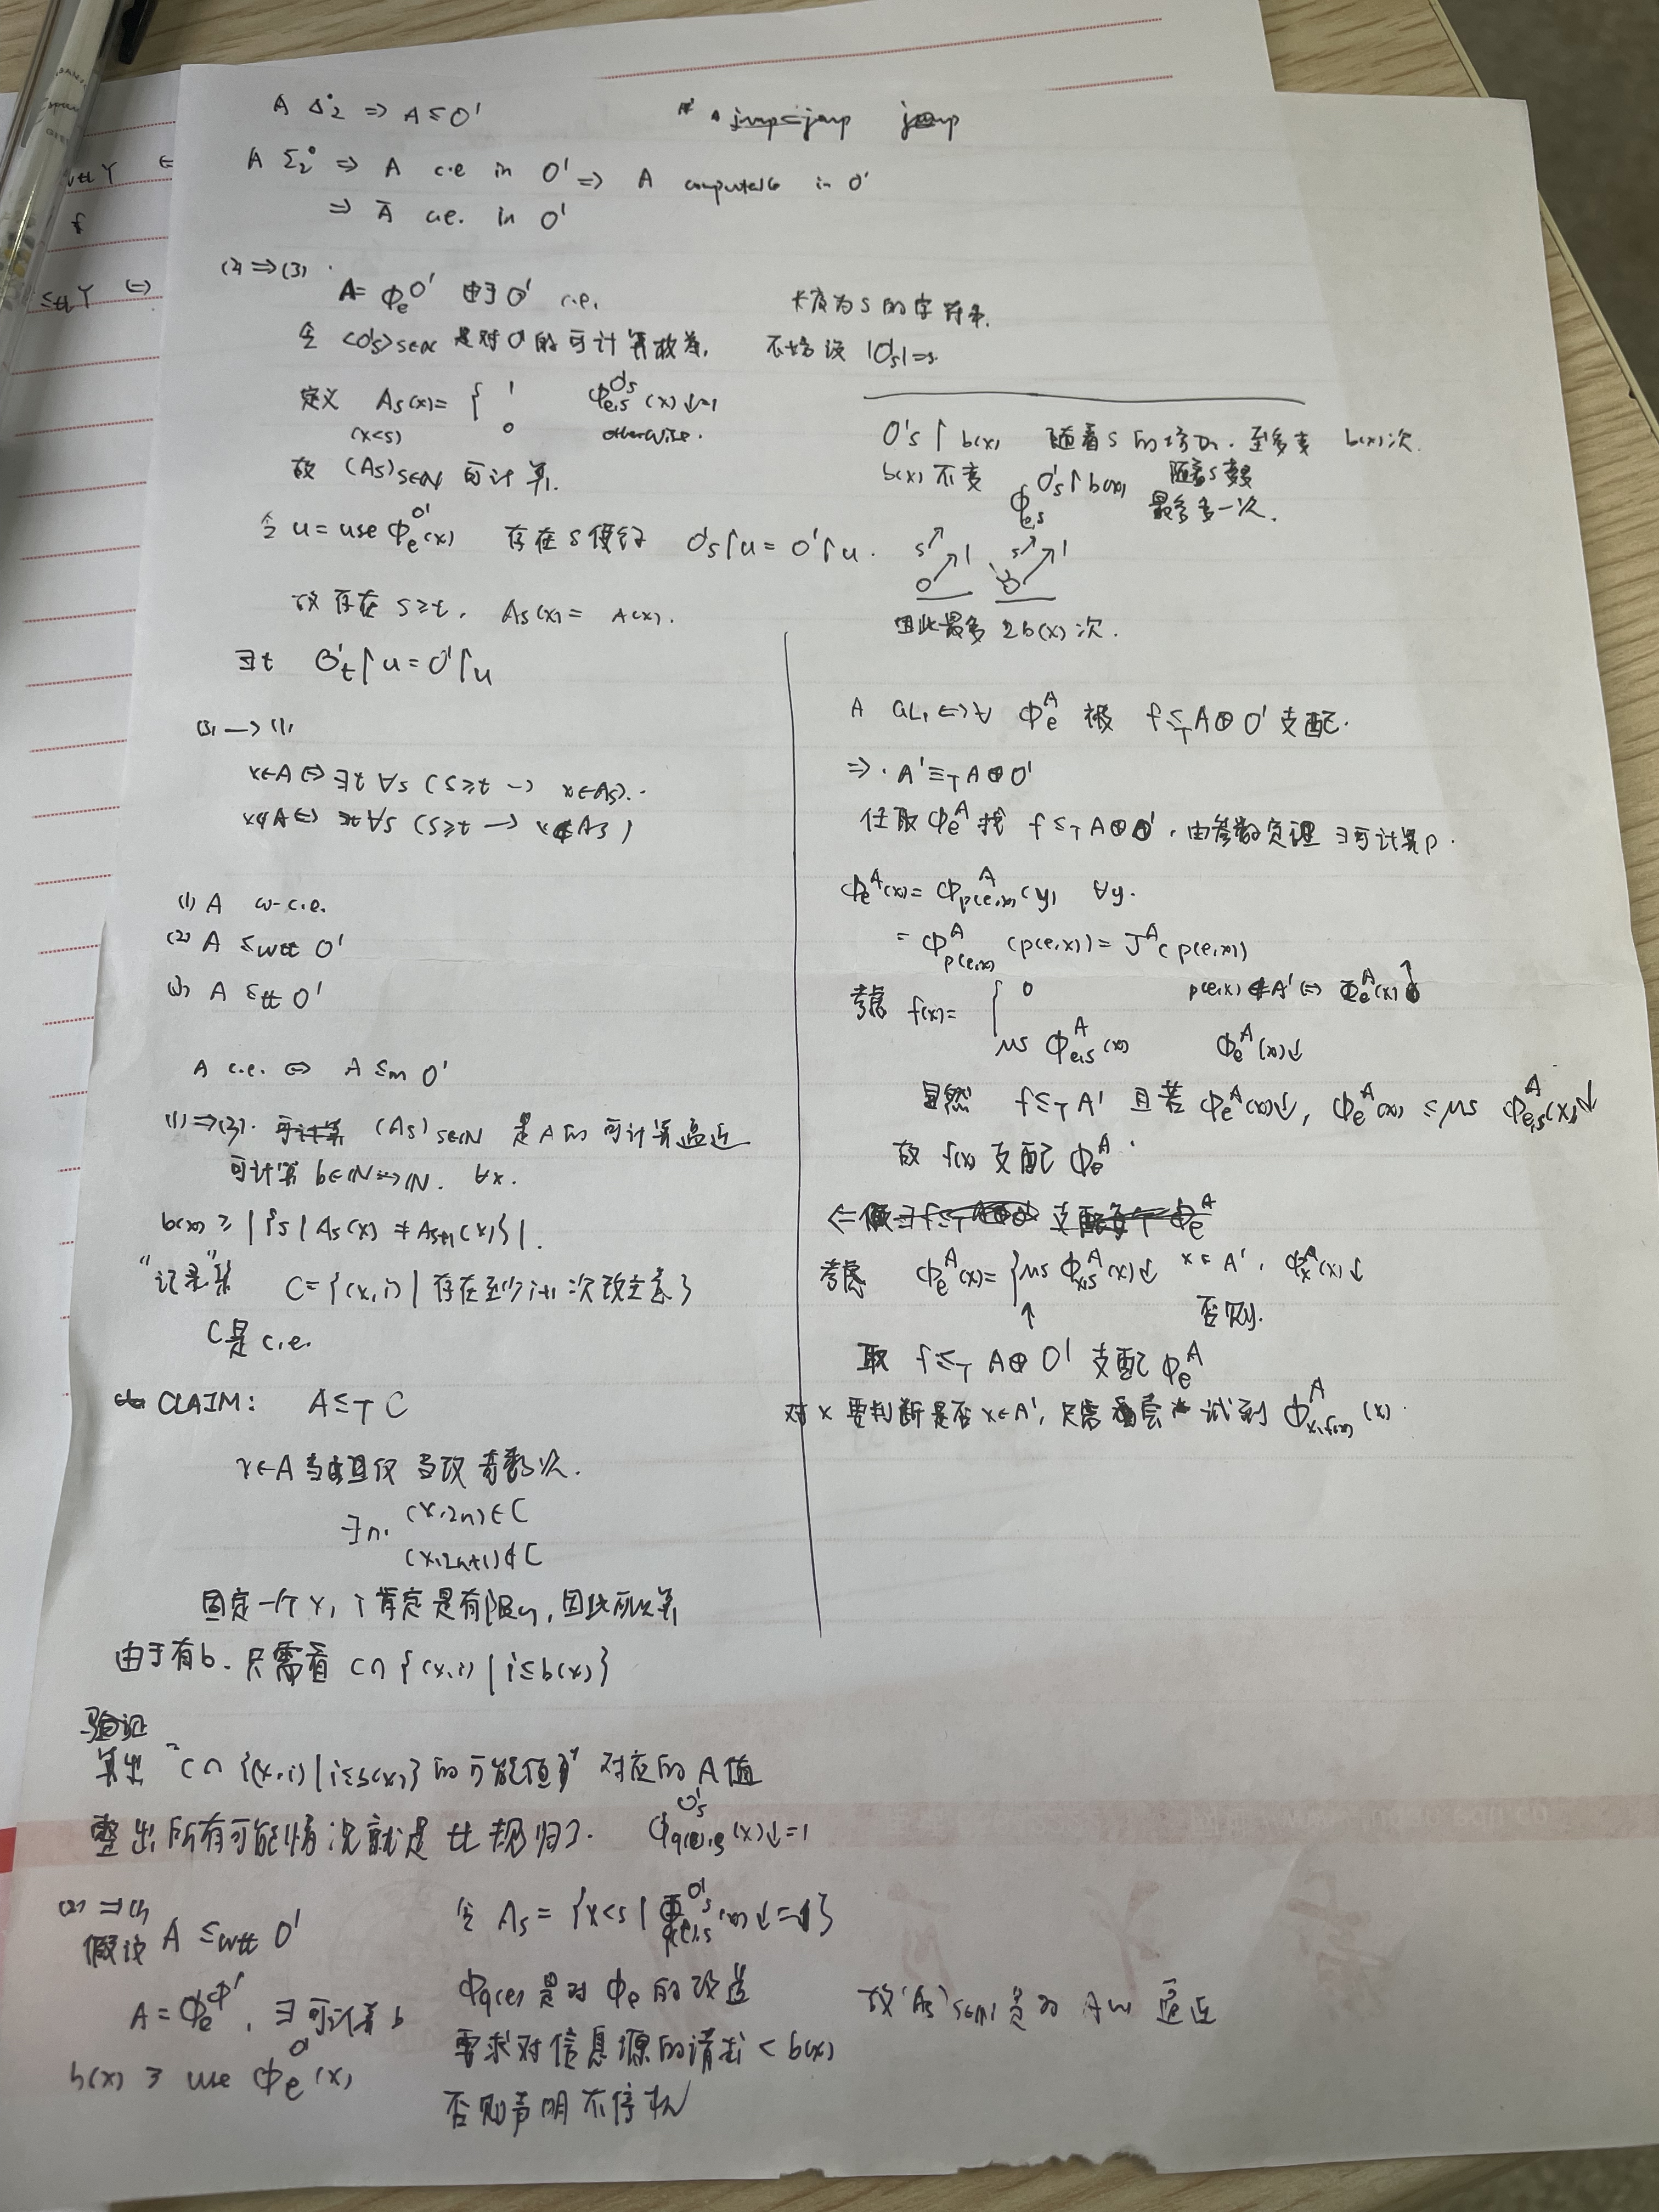
\includegraphics[width=.2\textwidth]{../images/DistributedAlgorithms/1.png}
\captionof{figure}{\label{10.2}The cycle of regions of a single user}
\end{center}

Each of the users \(U_i\), \(1\le i\le n\), is modelled as a state machine (formally, an \textbf{I/O
automaton}) that communicates with its agent process using the \(try_i\), \(crit_i\), \(exit_i\) and
\(rem_i\) actions:
\begin{center}
\includegraphics[width=.2\textwidth]{../images/DistributedAlgorithms/2.png}
\captionof{figure}{\label{10.3}External interface of user \(U_i\)}
\end{center}

We define a sequence of \(try_i\), \(crit_i\), \(exit_i\) and \(rem_i\) actions to be \textbf{well-formed} for
user \(i\) if it is a prefix of the cyclically ordered sequence
\(try_i,crit_i,exit_i,rem_i,try_i,\dots\). Then we require that \(U_i\) \textbf{preserve} the \textbf{trace property}
defined by the set of sequences that are well-ordered for user \(i\).
\section{Q\&A}
\label{sec:orgbfef732}
\begin{enumerate}
\item \ref{P1}. Need think.
\end{enumerate}
\end{document}
